\chapter{Differences}

\section{Supremum VS Maximum \cite{chatgpt}}\label{Supremum VS Maximum}

\begin{customTableWrapper}{2}
\begin{longtable}{|p{3cm}|p{6cm}|p{6cm}|}
    \hline
    \customTableHeaderColor
    \textbf{Aspect} & \textbf{Supremum} & \textbf{Maximum}\\ \hline
    \endfirsthead

    \hline
    \customTableHeaderColor
    \textbf{Aspect} & \textbf{Supremum} & \textbf{Maximum}\\ \hline
    \endhead

    \hline\endfoot
    \hline\endlastfoot

    \textbf{Inclusion in the Set} & The supremum of a set may or may not be an element of the set. & The maximum of a set must be an element of the set. \\
    \hline
    
    \textbf{Existence} & Every non-empty set bounded above in a complete ordered set (like the real numbers) has a supremum & A maximum exists only if there is at least one element that is greater than or equal to all other elements in the set\\
    \hline

    \textbf{Relationship} & If the maximum exists for a set S, it is equal to the supremum. In other words, if $max(S)$ exists, then $sup(S) = max(S)$ & If the maximum does not exist, the supremum is still defined as the least upper bound\\
    \hline

    \textbf{Example} & 
    \begin{minipage}{5cm}
        \vspace{0.1cm}
        $S = \dCurlyBrac{x \in R | x < 2}$ \\
        $sup(S) = 2$\\
        $max(S)$ doesn’t exist
        \vspace{0.1cm}
    \end{minipage} &
    \begin{minipage}{5cm}
        \vspace{0.1cm}
        $S = \dCurlyBrac{x \in R | x \leq 2}$ \\
        $sup(S) = 2$\\
        $max(S) = 2$
        \vspace{0.1cm}
    \end{minipage} \\
    \hline
\end{longtable}
\end{customTableWrapper}

\section{Infimum VS Minimum}\label{Infimum VS Minimum}
Similar to \fullref{Supremum VS Maximum}


%%%%%%%%%%%%%%%%%%%%%%%%%%%%%%%%%%%%%%%%%%%%%%%%%%%%%%%%%%%%%%%%%

\section{Covariate Shift (Data Shift) VS Concept Shift VS Prior Probability Shift (Label Shift) \cite{chatgpt}} \label{Covariate Shift (Data Shift) VS Concept Shift VS Prior Probability Shift (Label Shift)}

\begin{customTableWrapper}{1}
\begin{longtable}{|m{2cm}|m{4.5cm}|m{4.5cm}|m{4.5cm}|}
    \hline
    \customTableHeaderColor
    \textbf{Aspect} & \textbf{Covariate Shift (Data Shift)} & \textbf{Concept Shift} & \textbf{Prior Probability Shift (Label Shift)} \\ \hline
    \endfirsthead

    \hline
    \customTableHeaderColor
    \textbf{Aspect} & \textbf{Covariate Shift (Data Shift)} & \textbf{Concept Shift} & \textbf{Prior Probability Shift (Label Shift)} \\ \hline
    \endhead
    
    \hline\endfoot
    
    \hline\endlastfoot
    
    \textbf{Definition} & Change in the distribution of the input data (features) between training and test sets. & Change in the conditional distribution of the output given the input. & Change in the distribution of the output labels between training and test sets. \\ \hline
    
    \textbf{Cause} & Different data sources, sampling methods, or temporal changes affecting features. & Changes in the underlying relationship between features and labels, often due to evolving contexts or environments. & Variations in the frequency or proportion of different labels in the dataset over time. \\ \hline

    \textbf{Effect} & Model performance degradation due to misaligned feature distributions. & Model predictions become inaccurate because the learned relationships are no longer valid. & Bias in predicted label distribution if not accounted for, leading to misclassification. \\ \hline

    \textbf{Detection} & Comparing feature distributions (e.g., using statistical tests like KS test, histograms). & Analyzing the performance metrics over time or checking for changes in decision boundaries. & Comparing label distributions (e.g., using chi-square tests) or through domain knowledge. \\ \hline

    \textbf{Adjustment Techniques} & Reweighting samples, domain adaptation methods, or using robust models. & Regular retraining with updated data, transfer learning, or domain adaptation techniques. & Adjusting model outputs using methods like importance weighting, resampling, or calibration. \\ \hline

    \textbf{Example} & A retail model trained on summer sales data might perform poorly in winter due to changes in purchasing behavior. & A spam detection model might become less effective if spammers change tactics and the nature of spam emails evolves. & A medical diagnosis model might require adjustment if the prevalence of certain diseases changes in the population. \\ \hline

    \textbf{Relevance in Real-world Applications} & High when dealing with non-stationary environments or merging datasets from different sources. & High in dynamic environments where the relationship between input features and output labels can evolve. & High in situations with shifting class distributions, like seasonal changes or demographic shifts. \\ \hline

\end{longtable}
\end{customTableWrapper}

%%%%%%%%%%%%%%%%%%%%%%%%%%%%%%%%%%%%%%%%%%%%%%%%%%%%%%%%%%%%%%%%%

\section{Supervised Learning VS Unsupervised Learning VS Reinforcement Learning \cite{chatgpt,medium-numsmt2-rl-ch1-part-1}}\label{Supervised Learning VS Unsupervised Learning VS Reinforcement Learning}

\begin{customTableWrapper}{1.5}
\begin{longtable}{|p{1.6cm}|p{4.5cm}|p{4.5cm}|p{4.5cm}|}
    \hline
    \customTableHeaderColor
    \textbf{Aspect} & \textbf{Supervised Learning} & \textbf{Unsupervised Learning} & \textbf{Reinforcement Learning} \\
    \hline
    \endfirsthead

    \hline
    \customTableHeaderColor
    \textbf{Aspect} & \textbf{Supervised Learning} & \textbf{Unsupervised Learning} & \textbf{Reinforcement Learning} \\
    \hline
    \endhead
    
    \hline\endfoot
    \hline\endlastfoot
    
    \textbf{Training data} & Labeled data: Input-output pairs are provided for training. & Unlabeled data: Only input data is provided without corresponding output labels. & Trained from examples \& interaction with environment. \\
    \hline
    \textbf{Goal} & To learn a mapping from input data to output labels based on examples provided during training. & To find underlying patterns or structures in input data without explicit output labels. & To learn a policy that maximizes the cumulative reward by interacting with the environment. \\
    \hline
    \textbf{Feedback} & Direct feedback (error signal) is given during training based on the comparison between predicted output and actual output labels. & No explicit feedback based on labeled data; learning typically involves finding patterns or representations within the data. & Feedback is in the form of rewards or penalties from the environment. \\
    \hline
    \textbf{Examples} & Classification, regression tasks. & Clustering, association, dimensionality reduction. & Game playing, robotics, resource management. \\
    \hline
\end{longtable}
\end{customTableWrapper}

%%%%%%%%%%%%%%%%%%%%%%%%%%%%%%%%%%%%%%%%%%%%%%%%%%%%%%%%%%%%%%%%%

\section{Automatic Differentiation (AutoDiff) VS Backpropagation VS Chain Rule \cite{chatgpt}}\label{Automatic Differentiation (AutoDiff) VS Backpropagation VS Chain Rule}

\begin{customTableWrapper}{1.5}
\begin{longtable}{|p{2cm}|p{5cm}|p{3.5cm}|p{3.5cm}|}
    \hline
    \customTableHeaderColor
    \textbf{Aspect} & \textbf{Automatic Differentiation (AutoDiff)} & \textbf{Backpropagation} & \textbf{Chain Rule} \\
    \hline
    \endfirsthead
    
    \hline
    \customTableHeaderColor
    \textbf{Aspect} & \textbf{Automatic Differentiation (AutoDiff)} & \textbf{Backpropagation} & \textbf{Chain Rule} \\
    \hline\endhead
    
    \hline \endfoot
    
    \hline\endlastfoot
    
    \textbf{Definition} & Techniques for numerically evaluating derivatives of functions & Specific application of reverse mode AutoDiff for training neural networks & Calculus principle for computing derivatives of composed functions \\
    \hline

    \textbf{Modes} & Forward Mode, Reverse Mode & Reverse Mode & Not applicable \\
    \hline
    
    \textbf{Process} & Breaks down computation into elementary operations & Forward Pass, Loss Computation, Backward Pass & \(\dfrac{dy}{dx} = \dfrac{dy}{du} \cdot \dfrac{du}{dx}\) \\
    \hline
    
    \textbf{Used For} & Computing derivatives in general computational graphs & Training neural networks by computing gradients of the loss function & Computing derivatives of composed functions \\
    \hline
    
    \textbf{Efficiency} & Forward Mode: Efficient for few inputs, many outputs & Efficient for training neural networks due to large number of parameters & Applies to both AutoDiff and Backpropagation \\
    & Reverse Mode: Efficient for many inputs, few outputs & & \\
    \hline
    
    \textbf{Application} & Any function specified by a computer program & Neural network training (gradient-based optimization) & Fundamental concept in calculus \\
    \hline
    
\end{longtable}
\end{customTableWrapper}

%%%%%%%%%%%%%%%%%%%%%%%%%%%%%%%%%%%%%%%%%%%%%%%%%%%%%%%%%%%%%%%%%

\section{Batch Gradient Descent VS Mini-Batch Gradient Descent VS Gradient Descent (SGD) \cite{chatgpt}} \label{Batch Gradient Descent VS Mini-Batch Gradient Descent VS Gradient Descent (SGD)}

\begin{customTableWrapper}{2}
\begin{longtable}{|p{2.5cm}|p{4cm}|p{3.5cm}|p{3.5cm}|}
    \hline
    \customTableHeaderColor
    \textbf{Aspect} & \textbf{Batch Gradient Descent} & \textbf{Mini-Batch Gradient Descent} & \textbf{Gradient Descent (SGD)} \\
    \hline
    \endfirsthead
    
    \hline
    \customTableHeaderColor
    \textbf{Aspect} & \textbf{Batch Gradient Descent} & \textbf{Mini-Batch Gradient Descent} & \textbf{Gradient Descent (SGD)} \\
    \hline
    \endhead
    
    \hline\endfoot
    \hline\endlastfoot
    
    \textbf{Definition} & Updates parameters after computing the gradient on the entire dataset & Updates parameters after computing the gradient on a small batch of data & Updates parameters for each training example \\
    \hline

    \textbf{Update Frequency} & Low (after the entire dataset) & Medium (after each mini-batch) & High (after each example) \\
    \hline
    
    \textbf{Computation Cost/ Update} & High & Medium & Low \\
    \hline
    
    \textbf{Memory Usage} & High & Medium & Low \\
    \hline
    
    \textbf{Convergence Speed} & Slow & Fast & Fast \\
    \hline
    
    \textbf{Stability of Updates} & Stable (low variance) & Moderate (reduced variance) & Noisy (high variance) \\
    \hline
    
    \textbf{Convergence} & Guaranteed to decrease cost function & More stable convergence than SGD & May not converge to the global minimum \\
    \hline
    
    \textbf{Practical Use} & Suitable for smaller datasets & Suitable for large datasets & Suitable for very large datasets \\
    \hline
    
    \textbf{Hardware Optimization} & Limited & Allows for parallel processing & Limited \\
    \hline
    
    \textbf{Escape Local Minima} & Less likely & Yes (benefits of both SGD and Batch) & Yes (due to noisy updates) \\
    \hline
    
    \textbf{Example Size} & Entire dataset & Mini-batch (subset of dataset) & Single example \\
    \hline
    
    \textbf{Efficiency} & Low for large datasets & High, balancing efficiency and performance & High for very large datasets \\
    \hline

\end{longtable}
\end{customTableWrapper}

%%%%%%%%%%%%%%%%%%%%%%%%%%%%%%%%%%%%%%%%%%%%%%%%%%%%%%%%%%%%%%%%%

\section{Evaluation Metrics VS Criterion}\label{Evaluation Metrics VS Criterion}

\begin{customTableWrapper}{1}
\begin{longtable}{|p{2cm}|p{6cm}|p{6cm}|}
    \hline
    \customTableHeaderColor
    \textbf{Aspect} & \textbf{Evaluation Metrics} & \textbf{Loss Function (Criterion)} \\
    \hline
    \endfirsthead

    \hline
    \customTableHeaderColor
    \textbf{Aspect} & \textbf{Evaluation Metrics} & \textbf{Loss Function (Criterion)} \\
    \hline\endhead
    
    \hline\endfoot
    \hline\endlastfoot
    
    \textbf{Purpose} & Measure model performance on test or validation data after training. & Quantify error between predicted and actual values to guide optimization during training. \\
    \hline
    
    \textbf{Usage} & Assess model generalization and overall performance. & Internally used by optimizer to update model parameters based on prediction errors. \\
    \hline
    
    \textbf{Focus} & Reflects how well the model generalizes to new, unseen data. & Minimizing error on training data to improve model accuracy. \\
    \hline

    \textbf{Examples} & Accuracy, precision, recall, F1-score for classification tasks; RMSE, MAE for regression tasks. & MSE (Mean Squared Error), cross-entropy loss for classification tasks, etc. \\
    \hline
\end{longtable}
\end{customTableWrapper}

%%%%%%%%%%%%%%%%%%%%%%%%%%%%%%%%%%%%%%%%%%%%%%%%%%%%%%%%%%%%%%%%%

\section{Perceptron vs Artificial Neuron \cite{chatgpt}}\label{Perceptron vs Artificial Neuron}

\begin{customTableWrapper}{2}
\begin{longtable}{| m{3cm} | m{6cm} | m{6cm} |}
    
    \hline
    \customTableHeaderColor
    \textbf{Feature} & \textbf{Perceptron} & \textbf{Neuron in a Neural Network} \\
    \hline
    \endfirsthead
    
    \hline
    \customTableHeaderColor
    \textbf{Feature} & \textbf{Perceptron} & \textbf{Neuron in a Neural Network} \\
    \hline
    \endhead
    
    \hline
    \endfoot
    
    \hline
    \endlastfoot
    
    \textbf{Definition} & A type of artificial neuron used in binary classifiers. & A general computational unit in a neural network. \\
    \hline
    
    \textbf{Activation Function} & Uses a step function (binary output: 0 or 1). & Uses various activation functions (e.g., ReLU, sigmoid, tanh). \\
    \hline
    
    \textbf{Complexity} & Simple and linear. & Can be complex and non-linear. \\
    \hline
    
    \textbf{Learning Rule} & Uses the perceptron learning rule. & Uses more advanced learning rules (e.g., backpropagation). \\
    \hline
    
    \textbf{Output} & Binary output (0 or 1). & Continuous output, depending on the activation function. \\
    \hline
    
    \textbf{Applications} & Suitable for linear classification tasks. & Suitable for both linear and non-linear tasks. \\
    \hline
    
    \textbf{Historical Context} & One of the earliest models of an artificial neuron, introduced by Frank Rosenblatt in 1958. & Evolved from the perceptron, used in modern deep learning. \\
    \hline
    
    \textbf{Layers} & Typically used in single-layer models. & Used in multiple layers (deep networks). \\
    \hline

    \textbf{Expressive Power} & Limited to linearly separable problems. & Can model complex relationships and patterns. \\
    \hline

\end{longtable}
\end{customTableWrapper}

%%%%%%%%%%%%%%%%%%%%%%%%%%%%%%%%%%%%%%%%%%%%%%%%%%%%%%%%%%%%%%%%%

\section{Connectionism vs ANN \cite{chatgpt,arxiv-2405.04048}}\label{connectionism vs ann}

\begin{customTableWrapper}{1.5}
\begin{longtable}{|>{\raggedright\arraybackslash}p{3cm}|>{\raggedright\arraybackslash}p{6cm}|>{\raggedright\arraybackslash}p{6cm}|}
    
    \hline
    \customTableHeaderColor
    \textbf{Aspect} & \textbf{Connectionism} & \textbf{Artificial Neural Networks (ANNs)} \\
    \hline
    \endfirsthead
    
    \hline
    \customTableHeaderColor
    \textbf{Aspect} & \textbf{Connectionism} & \textbf{Artificial Neural Networks (ANNs)} \\
    \hline\endhead
    
    \hline\endfoot
    
    \hline\endlastfoot
    
    \textbf{Definition} & Theoretical framework for understanding the mind using interconnected networks of simple units. & Computational models inspired by brain's neural networks, used in machine learning. \\
    \hline
    
    \textbf{Scope} & Broad approach to cognition and brain function. & Specific computational implementations within connectionism. \\
    \hline
    
    \textbf{Focus} & Understanding cognitive processes and brain function. & Practical machine learning applications. \\
    \hline
    
    \textbf{Origins} & Cognitive science and psychology. & Efforts to mimic brain function for computational purposes. \\
    \hline
    
    \textbf{Key Concepts} & Neural networks, learning, parallel distributed processing, emergent properties. & Architecture (layers), activation functions, training (e.g., backpropagation), types (e.g., CNNs, RNNs). \\
    \hline
    
    \textbf{Learning} & Adjusting connection strengths based on experience. & Training involves adjusting weights to minimize prediction errors. \\
    \hline
    
    \textbf{Information Processing} & Parallel and distributed. & Parallel and distributed, with specific architectures (e.g., feedforward, convolutional). \\
    \hline
    
    \textbf{Applications} & Understanding perception, memory, language; modeling psychological phenomena. & Image and speech recognition, natural language processing, autonomous vehicles, medical diagnosis, financial forecasting. \\
    \hline
    
    \textbf{Theoretical Foundation} & Provides conceptual framework for cognition and brain modeling. & Empirical support for connectionist theories, demonstrating learning and task performance. \\
    \hline

    \textbf{Practical Implementation} & Conceptual approach with some computational models. & Implementations used in AI and machine learning. \\
    \hline
\end{longtable}
\end{customTableWrapper}

%%%%%%%%%%%%%%%%%%%%%%%%%%%%%%%%%%%%%%%%%%%%%%%%%%%%%%%%%%%%%%%%%

\section{Multilayer Perceptron (MLP) vs Artificial Neural Network (ANN)}\label{mlp vs ann}

\begin{customTableWrapper}{2}
\begin{longtable}{|>{\raggedright}m{4cm}|>{\raggedright}m{5cm}|>{\raggedright\arraybackslash}m{5cm}|}
    \hline
    \customTableHeaderColor
    \textbf{Feature} & \textbf{MLP (Multilayer Perceptron)} & \textbf{ANN (Artificial Neural Network)} \\
    \hline
    \endfirsthead

    \hline
    \customTableHeaderColor
    \textbf{Feature} & \textbf{Multilayer Perceptron (MLP)} & \textbf{Artificial Neural Network (ANN)} \\
    \hline
    \endhead

    \hline\endfoot
    
    \hline\endlastfoot
    
    \textbf{Definition} & A type of ANN with multiple layers & A broad category of machine learning models inspired by the human brain \\
    \hline
    
    \textbf{Structure} & Consists of input, hidden, and output layers & Can have various structures, including MLP, CNN, RNN, etc. \\
    \hline
    
    \textbf{Layers} & Always has at least one hidden layer & Can have any number of layers and types \\
    \hline
    
    \textbf{Neurons} & Fully connected layers of neurons & Can include different types of neurons (e.g., convolutional, recurrent) \\
    \hline
    
    \textbf{Training} & Typically trained with backpropagation & Can be trained with various algorithms depending on the type \\
    \hline
    
    \textbf{Usage} & Commonly used for classification and regression tasks & Used for a wide range of tasks including image recognition, natural language processing, etc. \\
    \hline
    
    \textbf{Complexity} & Generally less complex compared to other ANNs like CNNs and RNNs & Can range from simple to highly complex models \\
    \hline
    
    \textbf{Flexibility} & Less flexible compared to other ANN architectures & Highly flexible with many architectures available \\
\end{longtable}
\end{customTableWrapper}

%%%%%%%%%%%%%%%%%%%%%%%%%%%%%%%%%%%%%%%%%%%%%%%%%%%%%%%%%%%%%%%%%

\section{Model Parameter VS Model Hyperparameter \cite{chatgpt}}\label{Model Parameter VS Model Hyperparameter}

\begin{customTableWrapper}{2}
\begin{longtable}{|p{3cm}|p{6cm}|p{6cm}|}
    \hline
    \customTableHeaderColor
    \textbf{Aspect} & \textbf{Model Parameter} & \textbf{Model Hyperparameter} \\
    \hline
    \endfirsthead

    \hline
    \customTableHeaderColor
    \textbf{Aspect} & \textbf{Model Parameter} & \textbf{Model Hyperparameter} \\
    \hline
    \endhead

    \hline\endfoot
    \hline\endlastfoot

    \textbf{Setting/ changing} & Learned from the training data & Set before the training process \\ 
    \hline

    \textbf{Impact/ Significance} & Directly affect the predictions of the model & Affect the training process and the structure of the model \\
    \hline
\end{longtable}
\end{customTableWrapper}


%%%%%%%%%%%%%%%%%%%%%%%%%%%%%%%%%%%%%%%%%%%%%%%%%%%%%%%%%%%%%%%%%


\section{Underfitting VS Overfitting \cite{chatgpt}}\label{Underfitting VS Overfitting}

\begin{figure}[H]
    \centering
    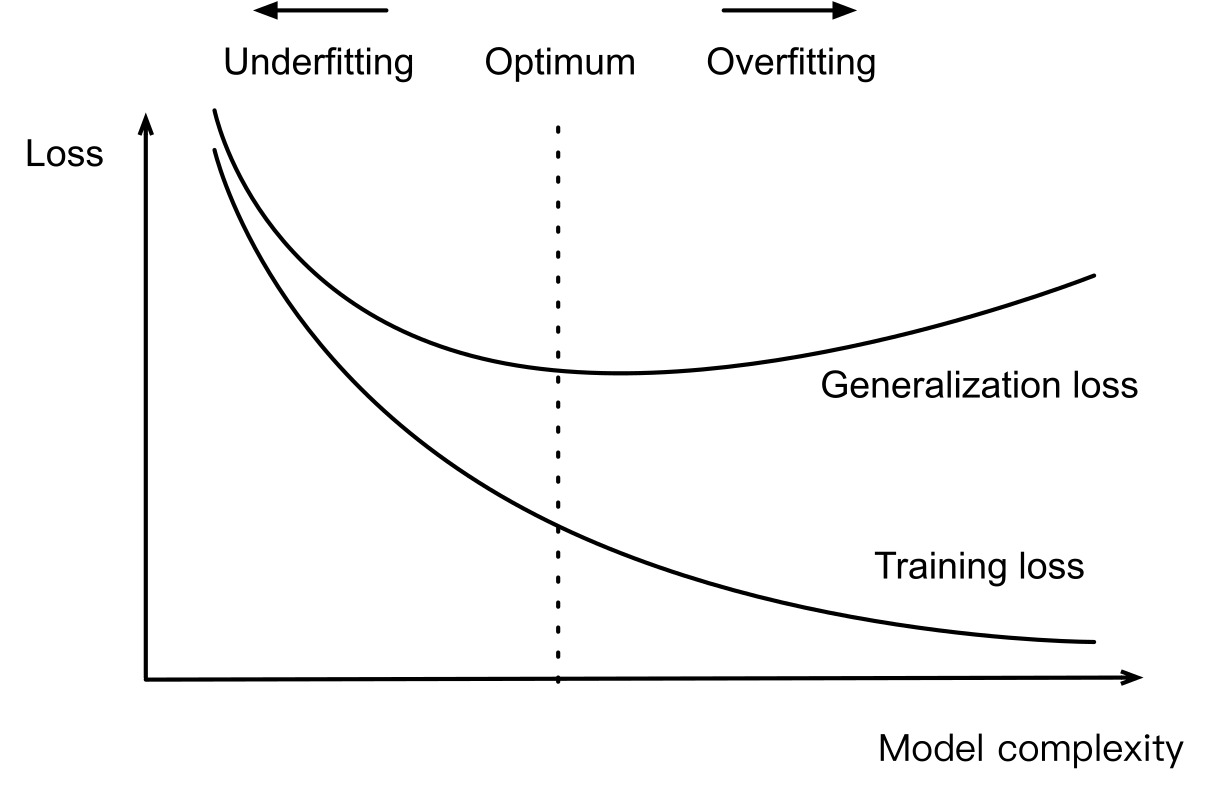
\includegraphics[width=\linewidth, height=4cm, keepaspectratio]{Pictures/deep_neural_networks/complexity-vs-error.jpg}
\end{figure}

\begin{customTableWrapper}{2}
\begin{longtable}{|p{3cm}|p{6cm}|p{6cm}|}
    \hline
    \customTableHeaderColor
    \textbf{Aspect} & \textbf{Underfitting} & \textbf{Overfitting} \\ 
    \hline
    \endfirsthead

    \hline
    \customTableHeaderColor
    \textbf{Aspect} & \textbf{Underfitting} & \textbf{Overfitting} \\ 
    \hline
    \endhead

    \hline\endfoot
    \hline\endlastfoot

    \textbf{Model’s complexity} & Underfitting occurs when a model is too simple to capture the underlying structure of the data & Overfitting occurs when a model is too complex and learns the noise in the training data rather than the actual underlying pattern\\
    \hline

    \textbf{Model’s Params} & model has too few parameters & model has too many parameters relative to the amount of training data \\
    \hline

    \textbf{Num of training iters} & model is not trained for enough iterations & reduce number of iters\\
    \hline

    \textbf{Training data performance} & Poor & Excellent\\
    \hline

    \textbf{Test data performance} & Poor & Poor \\
    \hline

    \textbf{Bias} & High & \\
    \hline

    \textbf{Variance} & & High \\
    \hline

    \textbf{Solution(s)} & \tableenumerate{
        \item \textbf{Increase model complexity}: Use a more complex model with more parameters
        
        \item \textbf{Train longer}: Ensure the model has sufficient time to learn from the data.
        
        \item \textbf{Feature engineering}: Create more relevant features that can help the model capture the underlying patterns
        
        \item \textbf{Reduce regularization}: Decrease the strength of regularization to allow the model to fit the training data better.
    } &
    \tableenumerate{
        \item \textbf{Simplify the model}: Use a less complex model with fewer parameters
        
        \item \textbf{Increase training data}: More data can help the model learn the underlying pattern rather than noise
        
        \item \textbf{Use regularization}: Techniques like L1 or L2 regularization can penalize large coefficients and prevent the model from becoming too complex
        
        \item \textbf{Cross-validation}: Use cross-validation techniques to ensure the model generalizes well to unseen data
        
        \item \textbf{Pruning}: In decision trees, remove branches that have little importance to reduce complexity
    }\\
    \hline


    \textbf{Risk Estimate} \cite{mfml-1} & & risk estimate from the training data $R_{emp}(f, X_{train}, y_{train})$ underestimates the expected risk $R_true(f)$\\
    \hline



\end{longtable}
\end{customTableWrapper}


%%%%%%%%%%%%%%%%%%%%%%%%%%%%%%%%%%%%%%%%%%%%%%%%%%%%%%%%%%%%%%%%%


\section{Likelihood VS Marginal likelihood (evidence) \cite{chatgpt}} \label{Likelihood VS Marginal likelihood (evidence)}

\begin{customTableWrapper}{1.5}
\begin{longtable}{|p{3cm}|p{6cm}|p{6cm}|}
    \hline
    \customTableHeaderColor
    \textbf{Aspect} & \textbf{Likelihood} & \textbf{Marginal Likelihood} \\
    \hline
    \endfirsthead

    \hline
    \customTableHeaderColor
    \textbf{Aspect} & \textbf{Likelihood} & \textbf{Marginal Likelihood} \\
    \hline
    \endhead

    \hline\endfoot
    \hline\endlastfoot

    \textbf{Definition} & The likelihood function measures how likely it is to observe the given data under different parameter values of a statistical model. It is a function of the model parameters, given the data. & The marginal likelihood, or evidence, is the probability of observing the data under a particular model, integrated over all possible parameter values weighted by their prior distribution. It serves as a measure of how well a model explains the observed data, considering both the likelihood and the prior distribution of the parameters. \\
    \hline

    \textbf{Formula} & $L(\theta;X) = P(X|\theta)$ & $P(X|M) = \int P(X|\theta,M) P(\theta|M) d\theta$ \\
    \hline

    \textbf{Usage} & 
    \tableenumerate{
        \item \textbf{Parameter Estimation}: In frequentist statistics, the maximum likelihood estimation (MLE) involves finding the parameter values that maximize the likelihood function.
        
        \item \textbf{Model Fitting}: It helps in fitting the model to the observed data by identifying the most probable parameters
    } &
    \tableenumerate{
        \item \textbf{Model Comparison}: In Bayesian model comparison, the marginal likelihood is used to compute the Bayes factor, which compares the relative plausibility of different models.
        
        \item \textbf{Model Selection}: It helps in selecting the model that best explains the observed data while incorporating the prior beliefs about the parameters.
    }\\
    \hline

    \textbf{Characteristics} &
    \tableenumerate{
        \item  It is not a probability distribution over the parameters but rather a measure of fit
        
        \item  It does not account for the prior distribution of parameters (in a Bayesian context)
    } &
    \tableenumerate{
        \item It accounts for both the fit of the model to the data (through the likelihood) and the complexity of the model (through the prior).
        
        \item It is a probability of the data given the model, hence it is used for comparing different models
    }\\
    \hline

    \textbf{Model Fitting} & likelihood is prone to overfitting & marginal likelihood is typically not as the model parameters have been marginalized out (i.e., we no longer have to fit the parameters) \\
    \hline

\end{longtable}
\end{customTableWrapper}


%%%%%%%%%%%%%%%%%%%%%%%%%%%%%%%%%%%%%%%%%%%%%%%%%%%%%%%%%%%%%%%%%


\section{Linked List VS Array \cite{geeksforgeeks/linked-list-vs-array}}\label{Linked List VS Array}

\begin{customTableWrapper}{2}
\begin{longtable}{|l|l|l|}
    \hline
    \customTableHeaderColor
    \textbf{Aspect} & \textbf{Array} & \textbf{Linked List} \\
    \hline
    \endfirsthead

    \hline
    \customTableHeaderColor
    \textbf{Aspect} & \textbf{Array} & \textbf{Linked List} \\
    \hline
    \endhead

    \hline\endfoot
    \hline\endlastfoot

    \textbf{Memory} & contiguous & not contiguous \\
    \hline

    \textbf{Size} & Fixed & Dynamic \\
    \hline

    \textbf{Memory allocation} & Compile time & Runtime \\
    \hline

    \textbf{Memory Usage} & Less & More \\
    \hline

    \textbf{Element Access} & Easy & Difficult\\
    \hline

    \textbf{Insertion \& Deletion operations} & Difficult & Easy \\
    \hline
\end{longtable}
\end{customTableWrapper}


%%%%%%%%%%%%%%%%%%%%%%%%%%%%%%%%%%%%%%%%%%%%%%%%%%%%%%%%%%%%%%%%

\section{Morphemes VS Lemma VS Stem \cite{chatgpt}} \label{Morphemes VS Lemma VS Stem}

\begin{customTableWrapper}{2}
\begin{longtable}{|p{2.5cm}|p{4cm}|p{4cm}|p{4cm}|}
    \hline
    \customTableHeaderColor
    \textbf{Aspect} & \textbf{Morpheme} & \textbf{Lemma} & \textbf{Stem} \\
    \hline
    \endfirsthead

    \hline
    \customTableHeaderColor
    \textbf{Aspect} & \textbf{Morpheme} & \textbf{Lemma} & \textbf{Stem} \\
    \hline
    \endhead

    \hline\endfoot
    \hline\endlastfoot

    \textbf{Definition} & The smallest grammatical units in a language carrying meaning; cannot be further divided. & The canonical or dictionary form of a word, encompassing all its inflected forms. & The form of a word to which affixes can be added, representing the core meaning. \\
    \hline

    \textbf{Function} & Constructs words and conveys grammatical relationships and meanings & Used for dictionary entries and linguistic analysis & Serves as the base for inflectional and derivational affixes \\
    \hline

    \textbf{Types} & Free Morphemes (can stand alone) and Bound Morphemes (cannot stand alone) & Single form representing all inflections of a word & Base form which can have derivational or inflectional affixes attached\\
    \hline

    \textbf{Word Analysis} & "unhappiness" = "un-" + "happy" + "-ness" & Lemma for "running", "ran", "runs" is "run" & Stem for "running", "runs" is "run" \\
    \hline
\end{longtable}
\end{customTableWrapper}


%%%%%%%%%%%%%%%%%%%%%%%%%%%%%%%%%%%%%%%%%%%%%%%%%%%%%%%%%%%%%%%%


\section{Ridge Regression (L2) VS Lasso Regression (L1)}\label{Ridge Regression VS Lasso Regression}

\begin{customTableWrapper}{2}
\begin{longtable}{|p{7cm}|p{7cm}|}
    \hline
    \customTableHeaderColor
    \textbf{Ridge Regression} & \textbf{Lasso Regression}\\
    \hline
    \endfirsthead
    
    \hline
    \customTableHeaderColor
    \textbf{Ridge Regression} & \textbf{Lasso Regression}\\
    \hline
    \endhead

    \hline\endfoot
    \hline\endlastfoot

    Shrinks the coefficients toward zero & Encourages some coefficients to be exactly zero\\
    \hline

    Adds a penalty term proportional to the sum of squared coefficients & Adds a penalty term proportional to the sum of absolute values of coefficients \\
    \hline

    Does not eliminate any features & Can eliminate some features \\
    \hline

    Suitable when all features are importantly & Suitable when some features are irrelevant or redundant\\
    \hline

    More computationally efficient & Less computationally efficient\\
    \hline

    Requires setting a hyperparameter & Requires setting a hyperparameter\\
    \hline

    Performs better when there are many small to medium-sized coefficients & Performs better when there are a few large coefficients\\
    \hline
\end{longtable}
\end{customTableWrapper}


%%%%%%%%%%%%%%%%%%%%%%%%%%%%%%%%%%%%%%%%%%%%%%%%%%%%%%%%%%%%%%


\section{Pearson’s Rho ($\rho_P$) VS Spearman’s Rho ($\rho_S$) VS Kendall’s Tau Correlation ($\tau_K$)} \label{Pearson’s Rho VS Spearman’s Rho VS Kendall’s Tau Correlation}

\begin{customTableWrapper}{1}
\begin{enumerate}
    \item They all describe a different aspect of the population and the difference can be quite large depending on the family of CDFs.

    \item product-moment correlation (Pearson’s Rho) provides a measure that is particularly suitable for linear associations between variables.

    \item data is normally distributed:
    \begin{enumerate}
        \item when the data are bivariate normally distributed, or when transformations can be applied that would make the data approximately bivariate normal, apply the product-moment estimator on the (transformed) data

        \item Pearson’s estimator $r_P$ is more efficient (i.e., has a smaller asymptotic variance) than Spearman’s estimator $r_S$
    \end{enumerate}

    \item data is \textbf{NOT} normally distributed:
    \begin{enumerate}
        \item Often Pearson’s product-moment estimator is immediately disqualified, since it is affected by transformations of the data. 

        \item prefer Kendall’s tau estimator over Spearman when the data is continuous, while we prefer Spearman’s rank when there are some ties
    \end{enumerate}

    \item For large datasets Kendall’s tau estimator is more efficient than Spearman’s rank correlation (the variances of $r_K$ and $r_S$ in the Fisher $z$-transformation. For Kendall’s tau this variance was $0.437/(n - 4)$, while it was at least $1/(n - 3)$ for Spearman’s rank correlation)

    \item when the data contain ties (i.e., values among the $x$ variable and/or values among the $y$ variable are equal), Spearman’s rank correlation has a smaller standard error than Kendall’s tau estimator

\end{enumerate}
\end{customTableWrapper}


%%%%%%%%%%%%%%%%%%%%%%%%%%%%%%%%%%%%%%%%%%%%%%%%%%%%%%%%%%%%%%


\section{PDF (Probability Density Function) VS PMF (Probability Mass Function) VS CDF (Cumulative Distribution Function)}\label{PDF (Probability Density Function) VS PMF (Probability Mass Function) VS CDF (Cumulative Distribution Function)}

\begin{customTableWrapper}{1}
\begin{longtable}{| m{2cm} | m{4cm} | m{4cm} | m{4cm} |}
    \hline
    \customTableHeaderColor
    \textbf{Aspect} & \textbf{PDF (Probability Density Function)} & \textbf{PMF (Probability Mass Function)} & \textbf{CDF (Cumulative Distribution Function)} \\
    \hline
    
    \textbf{Applies to} & Continuous random variables & Discrete random variables & Both continuous and discrete variables \\
    \hline
    
    \textbf{Definition} & Likelihood of the variable taking a specific value & Probability of the variable taking a specific value & Probability that the variable is less than or equal to a specific value \\
    \hline
    
    \textbf{Value Range} & Can be greater than 1 but integrates to 1 over all possible values & Between 0 and 1 & Between 0 and 1 \\
    \hline
    
    \textbf{Probability Calculation} & \(\int_{a}^{b} f_X(x) \, dx\) for interval \([a, b]\) & \(P(X = x)\) & \(P(X \leq x)\) \\
    \hline
    
    \textbf{Integral/ Sum Requirement} & Integral of the PDF over the entire range is 1 & Sum of the PMF over all possible values is 1 & \(\lim_{x \to -\infty} F_X(x) = 0\) and \(\lim_{x \to \infty} F_X(x) = 1\) \\
    \hline
    
    \textbf{Example} & \(f_X(x) = \frac{1}{\sqrt{2\pi}} e^{-x^2/2}\) & \(P(X = x) = \frac{1}{6}\) for a fair die & \(F_X(x) = \int_{-\infty}^{x} f_X(t) \, dt\) for continuous, \(F_X(x) = \sum_{x_i \leq x} P(X = x_i)\) for discrete \\
    \hline
\end{longtable}
\end{customTableWrapper}


%%%%%%%%%%%%%%%%%%%%%%%%%%%%%%%%%%%%%%%%%%%%%%%%%%%%%%%%%%%%%%


\section{Sum of Random Variables VS Mixture Distribution \cite{chatgpt}}\label{Sum of Random Variables VS Mixture Distribution}

\begin{customTableWrapper}{1}
\begin{longtable}{|p{2.5cm}|p{5cm}|p{5cm}|}
    \hline
    \customTableHeaderColor
    \textbf{Aspect} & \textbf{Sum of Random Variables} & \textbf{Mixture Distribution} \\
    \hline
    \endfirsthead
    
    \hline
    \customTableHeaderColor
    \textbf{Aspect} & \textbf{Sum of Random Variables} & \textbf{Mixture Distribution} \\
    \hline
    \endhead
    
    \hline
    \endfoot
    
    \hline
    \endlastfoot
    
    \textbf{Nature} & 
    Creates a new random variable by adding the original variables. & 
    Combines different distributions into one, considering the probabilities of each component. \\
    \hline
    
    \textbf{Definition} & 
    If \( X \) and \( Y \) are random variables, \( Z = X + Y \). The distribution of \( Z \) is derived from the distributions of \( X \) and \( Y \). & 
    A weighted sum of component distributions. For example, \( f(x) = \dsum_{i=1}^{k} \pi_i f_i(x) \), where \( \dsum_{i=1}^{k} \pi_i = 1 \). \\
    \hline
    
    \textbf{Independence} & 
    For independent random variables, the distribution of the sum is the convolution of their distributions. & 
    Does not require component distributions to be independent. \\
    \hline
    
    \textbf{Dependence} & 
    For dependent random variables, the sum's distribution depends on their joint distribution. & 
    Components can be dependent, but the mixture model itself does not model dependence between components. \\
    \hline
    
    \textbf{Central Limit Theorem} & 
    The sum of a large number of i.i.d. random variables tends to be normally distributed. & 
    Not directly related to the Central Limit Theorem. \\
    \hline
    
    \textbf{Applications} & 
    Used in contexts involving additive processes (e.g., total score, aggregated risk). & 
    Used in modeling populations with inherent heterogeneity (e.g., multi-modal distributions). \\
    \hline
    
    \textbf{Computation} & 
    Involves convolution for independent variables, which can be mathematically intensive. & 
    Involves weighted sums, and parameter estimation often uses methods like Expectation-Maximization (EM). \\
    \hline

\end{longtable}
\end{customTableWrapper}


%%%%%%%%%%%%%%%%%%%%%%%%%%%%%%%%%%%%%%%%%%%%%%%%%%%%%%%%%%%%%%


\section{Confidence Interval (CI) VS Asymptotic Confidence Interval (Asymptotic CI) \cite{chatgpt}} \label{Confidence Interval (CI) VS Asymptotic Confidence Interval (Asymptotic CI)}

\begin{customTableWrapper}{1}
\begin{longtable}{|p{3cm}|p{6cm}|p{6cm}|}
    \hline
    \customTableHeaderColor
    \textbf{Aspect} & \textbf{Confidence Interval (CI)} & \textbf{Asymptotic Confidence Interval (Asymptotic CI)} \\
    \hline
    \endfirsthead
    
    \hline
    \customTableHeaderColor
    \textbf{Aspect} & \textbf{Confidence Interval (CI)} & \textbf{Asymptotic Confidence Interval (Asymptotic CI)} \\
    \hline
    \endhead
    
    \hline\endfoot
    
    \hline\endlastfoot
    
    \textbf{Definition} & A range of values derived from sample data that is likely to contain the true parameter with a certain probability. & A confidence interval that becomes increasingly accurate as the sample size grows, often based on asymptotic properties. \\
    \hline

    \textbf{Basis} & Often derived from exact statistical methods or models, considering the sample size and distribution. & Derived from asymptotic theory, often assuming large sample sizes and normality of the estimator distribution. \\
    \hline
    
    \textbf{Sample Size} & Can be used for both small and large sample sizes, depending on the method. & Primarily used for large sample sizes where asymptotic properties are valid. \\
    \hline
    
    \textbf{Accuracy} & More accurate for small samples when exact methods are used. & Accuracy improves with larger sample sizes; may be less accurate for small samples. \\
    \hline
    
    \textbf{Distribution} & May use exact distributions (e.g., t-distribution) appropriate to the sample size. & Assumes that the estimator follows a normal distribution as sample size increases (Central Limit Theorem). \\
    \hline
    
    \textbf{Computation} & Can be more complex and involve exact calculations or simulations. & Often simpler and relies on large-sample approximations. \\
    \hline
    
    \textbf{Examples} & Exact t-interval for small sample sizes, exact binomial confidence intervals. & Approximate normal confidence interval for means, large-sample z-intervals. \\
    \hline
\end{longtable}
\end{customTableWrapper}


%%%%%%%%%%%%%%%%%%%%%%%%%%%%%%%%%%%%%%%%%%%%%%%%%%%%%%%%%%%%%%


\section{RCNN VS Fast RCNN VS Faster RCNN \cite{chatgpt}} \label{RCNN VS Fast RCNN VS Faster RCNN}

\begin{customTableWrapper}{1}
\begin{longtable}{|p{2.5cm}|p{3.5cm}|p{3.5cm}|p{3.5cm}|}
    \hline
    \customTableHeaderColor
    \textbf{Feature} & \textbf{RCNN} & \textbf{Fast RCNN} & \textbf{Faster RCNN} \\
    \hline
    \endfirsthead

    \hline
    \customTableHeaderColor
    \textbf{Feature} & \textbf{RCNN} & \textbf{Fast RCNN} & \textbf{Faster RCNN} \\
    \hline
    \endhead
    
    \hline\endfoot
    \hline\endlastfoot

    
    \textbf{Year Introduced} & 2013 & 2015 & 2015 \\
    \hline
    
    \textbf{Main Idea} & Region proposals + CNN & End-to-end training with ROI Pooling & End-to-end training with ROI Pooling and RPN \\
    \hline
    
    \textbf{Region Proposals} & Selective Search & Selective Search & Region Proposal Network (RPN) \\
    \hline
    
    \textbf{Training Steps} & Multi-stage: Pre-trained CNN + SVM classifiers + Bounding box regressors & Single-stage end-to-end & Single-stage end-to-end \\
    \hline
    
    \textbf{Speed} & Slow due to multiple forward passes & Faster due to shared computation & Fastest due to integrated RPN \\
    \hline
    
    \textbf{Complexity} & High (multiple models to train) & Moderate & Lower (integrated into a single network) \\
    \hline
    
    \textbf{Feature Extraction} & Uses a pre-trained CNN (e.g., AlexNet) & Uses a single CNN with ROI pooling & Uses a single CNN with ROI pooling and RPN \\
    \hline
    
    \textbf{Accuracy} & Good & Better than RCNN & Comparable to Fast RCNN, sometimes better \\
    \hline
    
    \textbf{Training Time} & Long & Shorter than RCNN & Shortest among the three \\
    \hline
    
    \textbf{Inference Time} & Long & Shorter than RCNN & Shortest among the three \\
\end{longtable}
\end{customTableWrapper}


%%%%%%%%%%%%%%%%%%%%%%%%%%%%%%%%%%%%%%%%%%%%%%%%%%%%%%%%%%%%%%


\section{Policy Iteration VS Value Iteration \cite{baeldung/cs/ml-value-iteration-vs-policy-iteration}} \label{Policy Iteration VS Value Iteration}

\begin{customTableWrapper}{2}
\begin{longtable}{|p{6cm}|p{6cm}|}
    \hline
    \customTableHeaderColor
    \textbf{Policy Iteration} & \textbf{Value Iteration} \\
    \hline

    Starts with a random policy & Starts with a random value function \\
    \hline
    
    Algorithm is more complex & Algorithm is simpler \\
    \hline
    
    Guaranteed to converge & Guaranteed to converge \\
    \hline
    
    Cheaper to compute & More expensive to compute \\
    \hline
    
    Requires few iterations to converge & Requires more iterations to converge \\
    \hline
    
    Faster & Slower \\
    \hline
\end{longtable}
\end{customTableWrapper}


%%%%%%%%%%%%%%%%%%%%%%%%%%%%%%%%%%%%%%%%%%%%%%%%%%%%%%%%%%%%%%


\section{Information Retrieval VS Data Retrieval \cite{gfg-what-is-ir}} \label{Information Retrieval VS Data Retrieval}

\begin{customTableWrapper}{1.5}
\begin{longtable}[H]{|p{7.5cm}|p{7.5cm}|}
    \hline
    \customTableHeaderColor
    \textbf{Information Retrieval} & \textbf{Data Retrieval}  \\
    \hline
    \endfirsthead

    \hline
    \customTableHeaderColor
    \textbf{Information Retrieval} & \textbf{Data Retrieval}  \\
    \hline\endhead
    
    \hline\endfoot
    \hline\endlastfoot
     
     \hline
     The software program that deals with the organization, storage, retrieval, and evaluation of information from document repositories particularly textual information.  & Data retrieval deals with obtaining data from a database management system such as ODBMS. It is A process of identifying and retrieving the data from the database, based on the query provided by user or application. \\
     \hline

     Retrieves information about a subject. & Determines the keywords in the user query and retrieves the data. \\
     \hline
     
     Small errors are likely to go unnoticed. & A single error object means total failure. \\
     \hline
     
     Not always well structured and is semantically ambiguous. & Has a well-defined structure and semantics. \\
     \hline
     
     Does not provide a solution to the user of the database system. & Provides solutions to the user of the database system. \\
     \hline
     
     The results obtained are approximate matches. & The results obtained are exact matches. \\
     \hline
     
     Results are ordered by relevance. & Results are not ordered by relevance.\\
     \hline
     
     It is a probabilistic model. & It is a deterministic model.\\
     \hline
\end{longtable}
\end{customTableWrapper}


%%%%%%%%%%%%%%%%%%%%%%%%%%%%%%%%%%%%%%%%%%%%%%%%%%%%%%%%%%%%%%


\section{Policy Iteration VS Generalized Policy Iteration (GPI)}\label{Policy Iteration VS Generalized Policy Iteration (GPI)}

\begin{customTableWrapper}{1.5}
\begin{longtable}{|l|p{5cm}|p{5cm}|}
    \hline
    \customTableHeaderColor
    \textbf{Aspect} & \textbf{Policy Iteration} & \textbf{Generalized Policy Iteration (GPI)} \\
    \hline
    
    \textbf{Steps} & 
    \tableitemize{
        \item Policy Evaluation
        \item Policy Improvement
    } & 
    \tableitemize{
        \item Policy Evaluation (or Estimation)
        \item Policy Improvement (or Control)
    } \\
    \hline
    
    \textbf{Step Completion} & 
    Each step is performed to completion before moving to the next. & 
    Steps can be interleaved and performed partially. \\
    \hline
    
    \textbf{Flexibility} & 
    Less flexible, as it requires full policy evaluation before improvement. & 
    More flexible, allowing for incremental and simultaneous evaluation and improvement. \\
    \hline
    
    \textbf{Convergence} & 
    Has well-defined convergence criteria. & 
    Requires more sophisticated analysis for convergence, especially with incremental or stochastic steps. \\
    \hline
    
    \textbf{Practical Use} & 
    Suitable for small state and action spaces where exact solutions are feasible. & 
    Suitable for large-scale or complex problems where exact evaluation and improvement are infeasible. \\
    \hline

    \textbf{Example Algorithms} & 
    Classical Policy Iteration & 
    Q-learning, SARSA \\
    \hline
\end{longtable}
\end{customTableWrapper}


%%%%%%%%%%%%%%%%%%%%%%%%%%%%%%%%%%%%%%%%%%%%%%%%%%%%%%%%%%%%%%

\section{Attention VS Attention Pooling \cite{chatgpt}} \label{Attention VS Attention Pooling}

\begin{customTableWrapper}{1.5}
\begin{longtable}{|p{2cm}|p{5cm}|p{5cm}|}
    \hline
    \textbf{Aspect} & \textbf{Attention} & \textbf{Attention Pooling} \\
    \hline
    \endfirsthead
    
    \hline
    \textbf{Aspect} & \textbf{Attention} & \textbf{Attention Pooling} \\
    \hline
    \endhead
    
    \hline
    \endfoot
    
    \hline
    \endlastfoot

    \textbf{Purpose} & Focuses on relevant parts of the input dynamically. & Aggregates information into a single vector. \\
    \hline
    
    \textbf{Usage} & Used in tasks like translation to decide focus points. & Used to summarize multiple inputs into one representation. \\
    \hline
    
    \textbf{Operation} & Calculates attention weights for each input element. & Applies attention weights to create a weighted sum. \\
    \hline
    
    \textbf{Context} & Context-dependent; changes dynamically with each step. & Provides a fixed summary based on computed weights. \\
    \hline
    
    \textbf{Example} & Transformer models focusing on different words during decoding. & BERT model creating a single vector representation of a sentence. \\
    \hline

    \textbf{Output} & Weighted context vectors for each input element. & A single vector summarizing the input set. \\
    \hline

\end{longtable}
\end{customTableWrapper}















